\chapter{Introducion} \label{ch:Introduction}
\section{Interferon-Induced Proteins with Tetratricopeptide Repeats} \label{sec:Interferon-Induced Proteins with Tetratricopeptide Repeats}
The interferon-induced proteins with tetratricopeptide repeats (\textit{IFIT}) gene family are interferon-stimulated genes (ISGs) that are activated early in antiviral response. In unstimulated cells, with the exception of some myeloid cell subsets, they are barely detectable; however, upon viral infection, their translated products become some of the most abundant proteins in the cell \cite{Diamond2013TheProteins}. \textit{IFITs} are conserved in higher animals yet absent in the genomes of plants, insects, and yeast. 

With regards to their genomic composition, they are composed of two exons, the first encoding the ATG, two additional nucleotides and a 5' untranslated region (UTR), with the second exon containing the rest of the coding sequence and 3' UTR \cite{deVeer1998IFI60/ISG60/IFIT4Genes}. Most of the IFIT family gene members contain multiple copies of specific sequences in their promoter regions called interferon-stimulated response elements (IRSE), which are targets for downstream effectors of the interferon signalling cascade, enabling the fast activation of IFIT gene transcription \cite{Lou2009IFR-9/STAT2STAT1}. Both human and bovine IFIT locus confronts to the same genomic organisation, in terms of \textit{IFIT} gene orientation and order, and contains either two or three ISRE regions proceeding each of the IFIT genes \cite{Liu2013Lineage-SpecificFamily}.

Most mammalian IFIT genes are categorised into 4 subgroups named IFIT1, IFIT2, IFIT3, and IFIT5 all with clear orthologous relationships \cite{Sarkar2004NovelGenes}. Primates, along with some other mammalian species have a duplication of IFIT1 called IFIT1B, which lacks the ISRE in its gene promoter regions, and thus effectivelly only act as a pseudogene. Several rodents including mice and rats have lost the IFIT1 and IFIT5 genes and have duplications of IFIT1B and IFIT3 \cite{Daugherty2016Evolution-guidedMammals.} resulting in IFIT1B (typically referred to as IFIT1), IFIT1B-like gene 1, IFIT1B-like 2 gene, IFIT3 and IFIT3B genes. In contrast, avian species have lost most IFIT genes, with only one left resembling human IFIT5 \cite{Liu2013Lineage-SpecificFamily}. These variations in IFIT gene numbers are most probably the result of differing evolutionary pressures posed by different viruses affecting their respective host species, although it is evident that maintaining IFIT genes in the genome must be beneficial. 

\subsection{Routes of \textit{IFIT} Expression Activation} \label{subsec:Routes of IFIT Expression Activation}
\subsubsection{Interferon Signalling} \label{Interferon Signalling}
\textit{IFIT} induction can be achieved by activating several arms of the innate immune system (Figure \ref{fig:Pathways Inducing ISG mRNA Production.}). The strongest inducers are type I interferons, such as Interferon alpha and beta (IFN\(\alpha\)/\(\beta\)).  Their signalling is mediated via activation of IFN\(\alpha\)/\(\beta\) receptor and the subsequent downstream Janus kinase (JAK), and Signal transducer and activator of transcription (STAT) signal transduction. As a result, interferon-stimulated gene factor 3 (ISGF3), consisting of phosphorylated STAT1 and STAT2 proteins bound to interferon regulatory factor (IRF) IRF9, translocates to the nucleus, binds to the ISRE in the IFIT promoters and induces their transcription \cite{Der1998IdentificationArrays, Mesev2019DecodingInfection, Schoggins2011Interferon-stimulatedFunctions}. 

\subsubsection{Pattern Recognition Receptors} \label{Pattern Recognition Receptors}
Another arm of \textit{IFIT} activation is mediated through several pattern recognition receptors (PRRs), which can recognise various pathogen-associated molecular patterns (PAMPs). \textit{IFITs} have been reported to be induced by bacterial PAMPs such as lipopolysaccharide (LPS) from Neisseria meningitidis via activation of Toll-like receptor (TLR) 4 \cite{Zhou2013InterferonDefense.}. Interestingly, TLR4 has also been observed to be activated by the glycoprotein of respiratory syncytial virus (RSV) \cite{Funchal2015RespiratoryNeutrophils}. Other TLRs such as TLR3, TLR7, and TLR9 are capable of sensing PAMPs in the form of foreign nucleic acids in the endosomes. TLRs then interact with their adaptor proteins to in turn activate IRF3, IRF7, and nuclear factor kappa B (NF\(\kappa\)B), all of which have the capability to induce \textit{IFIT} family genes \cite{Diamond2013TheProteins}. These pathways are often prevalent in lymphocytes, monocytes, and mast cells; however, cytosolic nucleic acid sensors are functional in a broader subset of cells \cite{Ablasser2011WhereFit}.

\begin{figure}
    \centering
    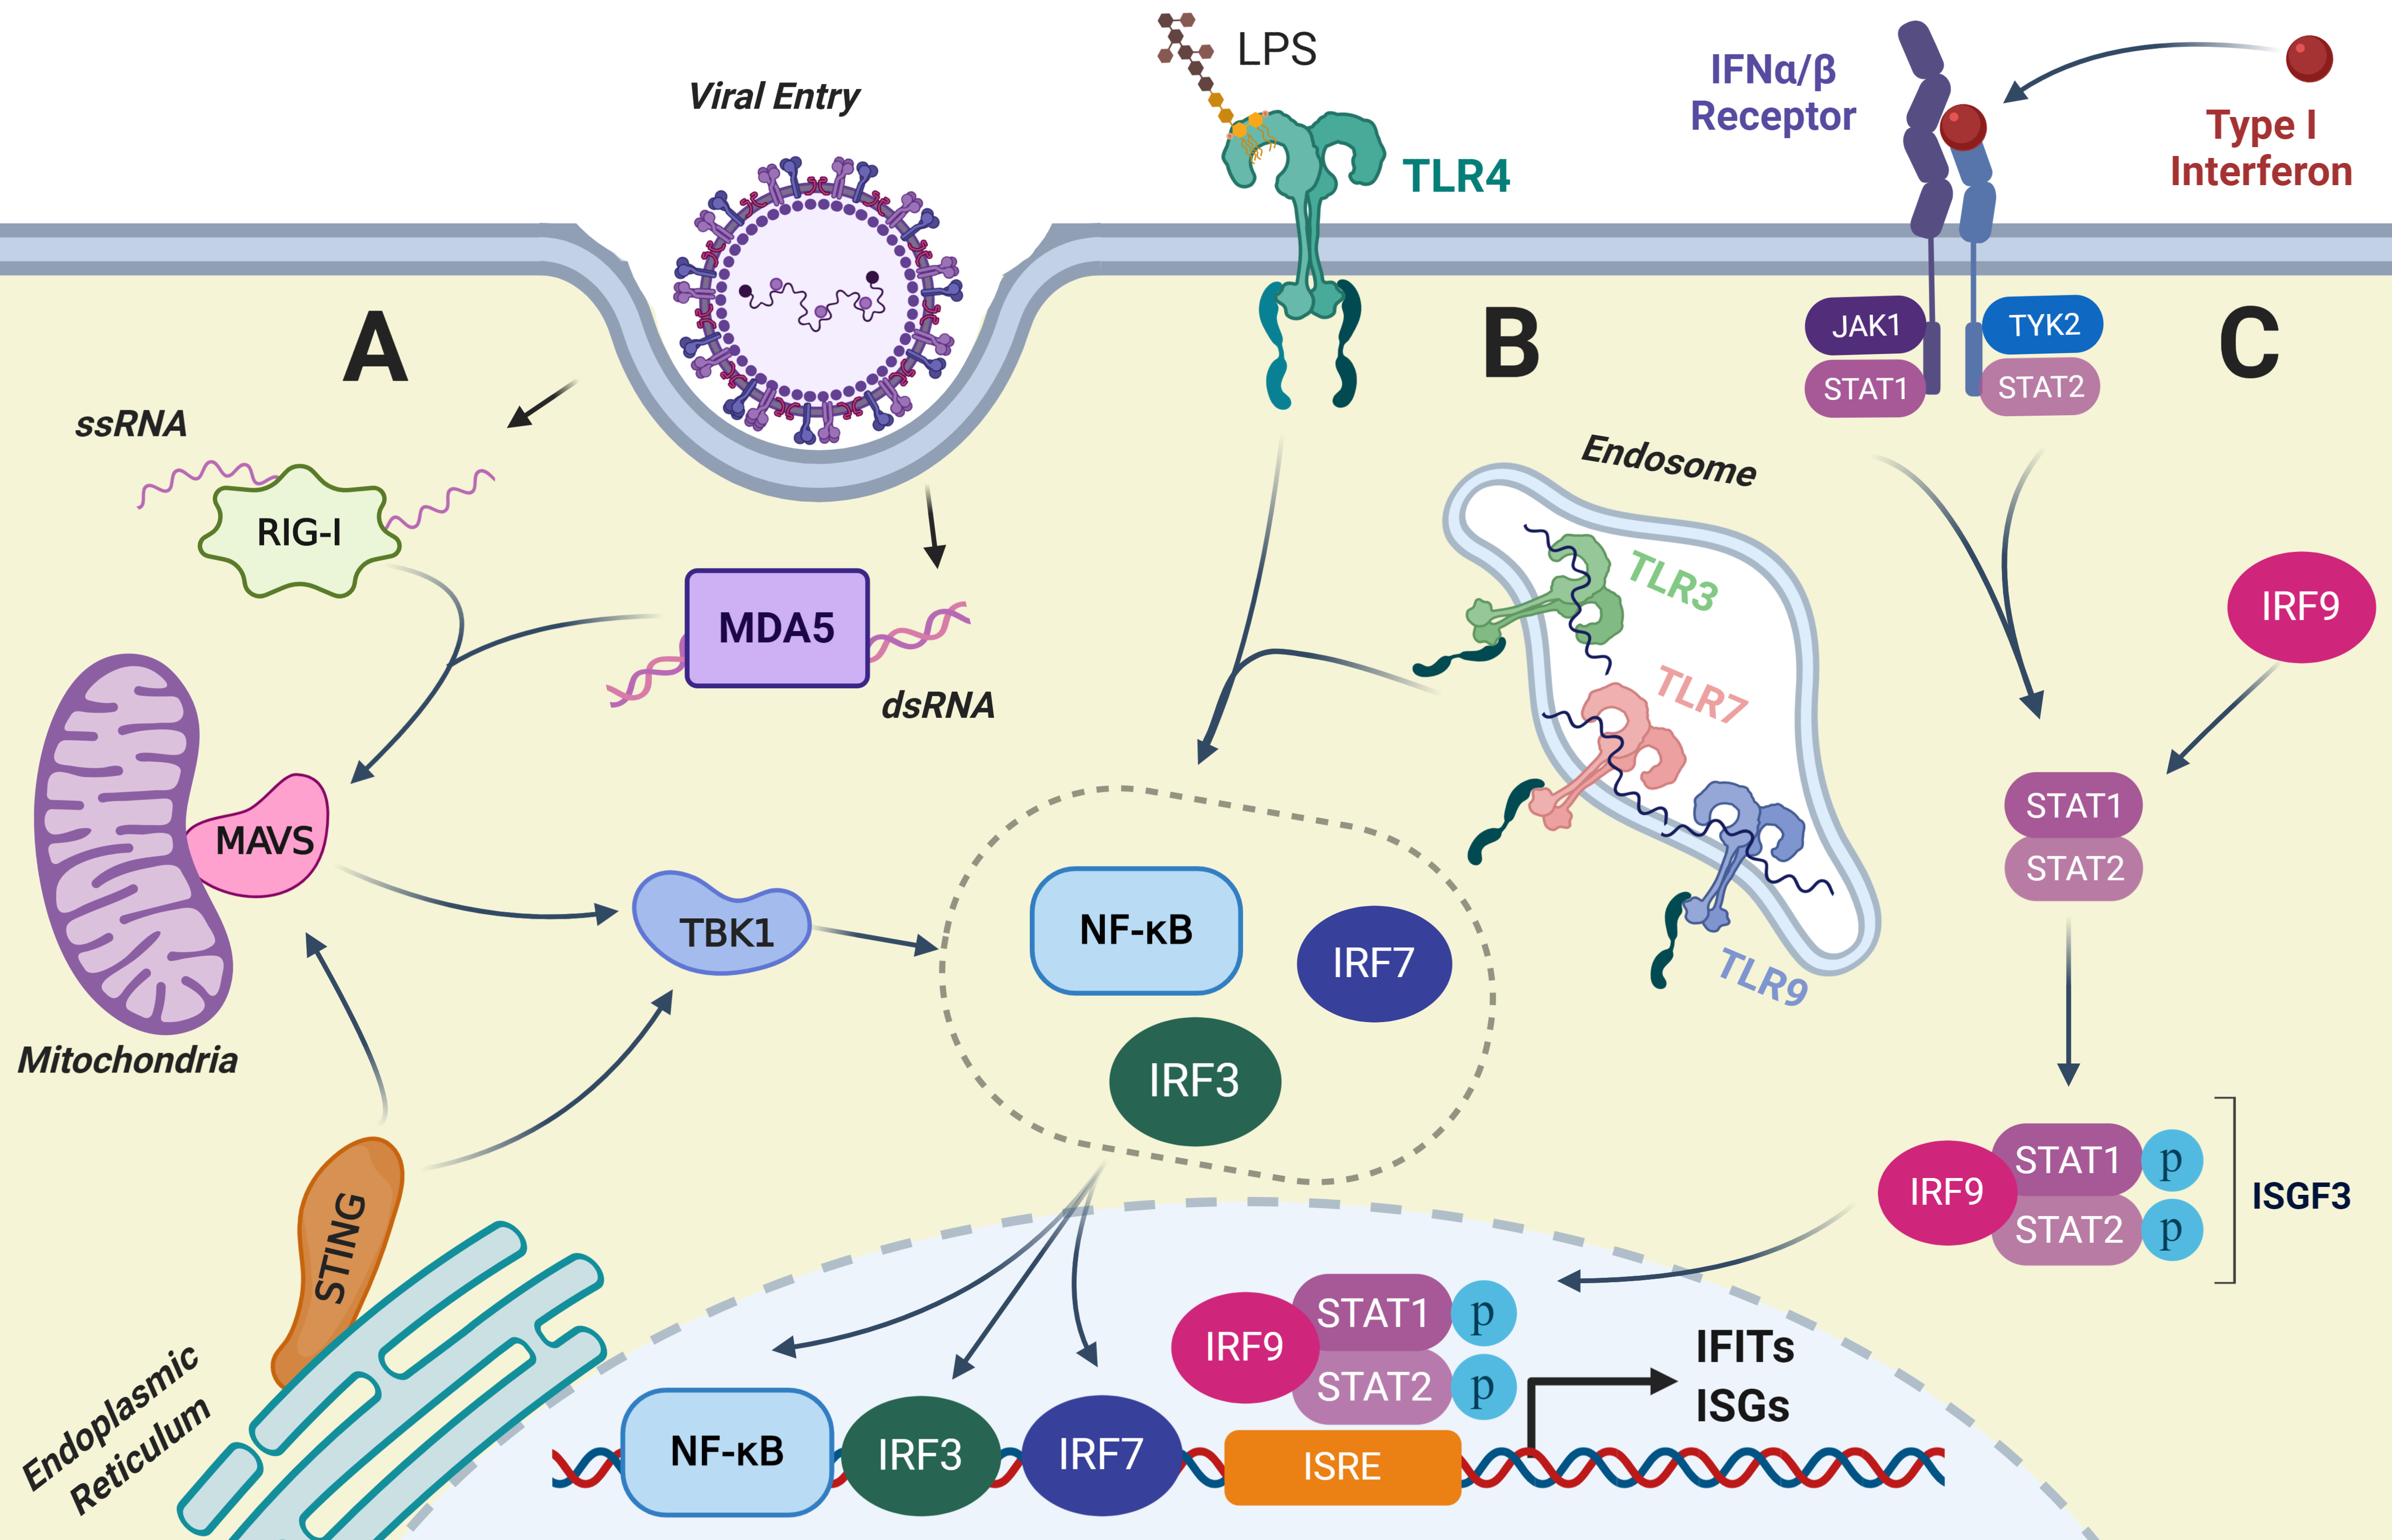
\includegraphics[width=1\linewidth]{04. Introduction//Figs/01. IFIT transcription activation figure.png}
    \caption[Pathways Inducing ISG mRNA Production.]{\textbf{Pathways Inducing ISG mRNA Production.} Three routes of ISGs transcription induction are depicted. Pathway A shows virus releasing its genome upon its entry and subsequent foreign nucleic acid detection by cytosolic sensors RIG-I and MDA5. These detect single-stranded and double-stranded RNA respectively. Both activate MAVS, which in turn activates TBK1. STING protein facilitates this activation by enhancing MAVS and TBK1 interaction. Pathway B shows PAMP detection by TLR receptors. TLR4 recognises LPS in the extracellular space while TLR3, TLR7, and TLR9 detect foreign nucleic acids in endosomes. TBK1, as well as TLR activation, leads to the translocation of activated IRF3, IRF7, and NF\(\kappa\)B into the nucleus where they promote ISGs transcription activation. Pathway C depicts type 1 interferon signalling pathway. IFN\(\alpha\)/\(\beta\) receptor activation leads to STAT1 and STAT2 activation. Further addition of IRF9 forms ISGF3 complex, which translocates into the nucleus onto ISRE and promotes ISGs transcription activation. ISG, interferon-stimulated genes; RIG-I, retinoic acid-inducible gene-I; MDA5, melanoma differentiation-associated gene 5; MAVS, mitochondrial antiviral signalling protein; TBK1, TANK-binding kinase 1; STING, stimulator of interferon genes; PAMP, pathogen-associated molecular pattern; TLR, toll-like receptor; IRF, interferon regulatory factor; NF\(\kappa\)B, nuclear factor kappa B; IFN, interferon; STAT, signal transducer and activator of transcription; ssRNA, single-stranded RNA; dsRNA, double-stranded RNA; ISGF, interferon-stimulated gene factor; ISRE, interferon-stimulated response elements. The figure was adapted from Diamond and Farzan, (2013) \cite{Diamond2013TheProteins} and Natalya Odoardi's BioRender template. Created with BioRender.com.}
    \label{fig:Pathways Inducing ISG mRNA Production.}
\end{figure}

\subsubsection{Cytosolic Nuclec Acid Sensors} \label{Cytosolic Nuclec Acid Sensors}
Cytosolic RNA sensors include melanoma differentiation-associated gene 5 (MDA5) and retinoic acid-inducible gene I (RIG-I) \cite{Vladimer2014IFITs:Proteins}. Both signal through mitochondrial antiviral signalling protein (MAVS), which in turn activates IRF3, IRF7, and NF\(\kappa\)B as their downstream effectors \cite{Ashley2019Interferon-IndependentCytomegalovirus}. In order to prevent activation by cellular RNA molecules, a precise RNA-recognition mechanism has to be conducted by the sensors. While MDA5 senses long double-stranded RNA (dsRNA) \cite{Brisse2019ComparativeMDA5}, RIG-I is able to sense differences in the 5' RNA modifications \cite{Schlee2016DiscriminatingSensing}. During mRNA maturation in higher eukaryotes, 7-methyl guanosine (m7G) is connected by a 5'- 5' triphosphate bridge, which is referred to as capping \cite{Devarkar2016StructuralRIG-I, Ramanathan2016MRNAApplications}. Several viruses carry uncapped, 5'-triphosphorylated (5'-PPP) or incompletely capped RNA (cap 0), whereas host animals possess cap-1 and cap-2 mRNA moieties \cite{Choi2018ACaps}, which are all depicted in Figure \ref{fig:Overview of 5'RNA Modifications.}. \textit{IFITs} can be activated by several signal transduction pathways, each with its own inducers and kinetics. A cross-play of these pathways is what in turn orchestrates IFIT response during viral infection.

\begin{figure}
    \centering
    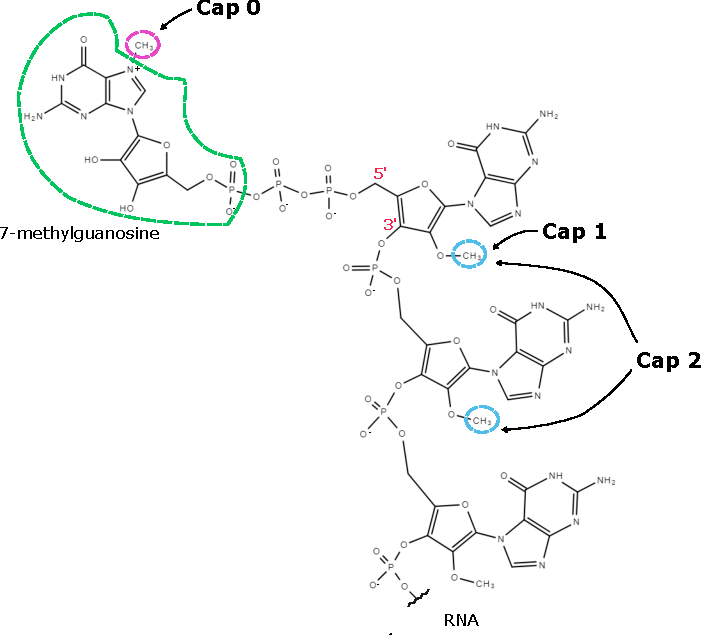
\includegraphics[width=0.75\linewidth]{04. Introduction//Figs/02. 5-RNA Modifications.pdf}
    \caption[Overview of 5'RNA Modifications.]{\textbf{Overview of 5'RNA Modifications.} Mature mRNA is displayed. Higher eukaryotes modify their mRNA by the initial addition of guanosine (blue) via 5' - 5' triphosphate bridge to the 5' end. Subsequently, the guanosine is methylated into 7-methylguanosine (green) and this modification is referred to as Cap0 structure. Furthermore, the first 2 bases of RNA can be methylated (red) and make either Cap1 or Cap2 structural modifications (yellow arrows). The figure was adapted from Picard-Jean, 2013 \cite{Picard-Jean2013RNAGenomes}.}
    \label{fig:Overview of 5'RNA Modifications.}
\end{figure}

\subsection{Structural Features of IFIT Proteins} \label{subsec:Structural Features of IFIT Proteins}
IFITs are composed of multiple copies of tetratricopeptide repeats (TPR). These are motifs comprised of 3-16 tandem repeats of 34 amino acids, which adopt helix-turn-helix confirmations \cite{DAndrea2003TPRHelix}. TPRs are conserved in all species from bacteria through plants to higher animals and are commonly found in scaffolding proteins \cite{Vladimer2014IFITs:Proteins}. IFIT TPRs are comprised of degenerate sequences meaning the conservation of the motif is limited. This allows different IFIT proteins to have a broader profile of protein interactors while still maintaining the overall conformation \cite{Fensterl2015Interferon-InducedPathogenesis}. IFIT proteins are often subjected to post-translational modifications such as ubiquitination or ISGylation (addition of small IFN-induced ubiquitin-like proteins), which may alter IFIT stability and function.

\subsubsection{IFITs and Their Interaction with RNA} \label{IFITs and Their Interaction with RNA}
IFIT1 and IFIT5 both form a positively charged channel with an affinity for 5' ends of single-stranded RNA (ssRNA) molecules in a sequence non-specific manner. IFIT5 can accommodate 5'PPP RNA and effectively acts as a sensor for these molecules \cite{Abbas2013StructuralProteins, Pichlmair2011IFIT1RNA}. On the other hand, IFIT1 can accommodate m7G, but certain residues inside its channel prevent efficient binding of cap1 and cap2 moieties \cite{Diamond2014IFIT1:Translation, Mears2018BetterResponse}. Through these interactions they can effectively discriminate between self and non-self RNA moieties. IFIT2 is also capable of RNA binding, albeit independent on the 5'-capping state. The C terminals of IFIT2 homo-dimer create a super-helical structure with a positively-charged nucleotide-binding channel on its inner surface, which was observed to bind to AU-rich RNA molecules \cite{Yang2012CrystalMechanisms}. Mechanistic studies identified IFIT2 binding to mRNAs as important to prevent ribosomal pausing and thus increasing the transnational efficiency of IFIT2-bound mRNAs, a process which has been observed to be hijacked by influenza A virus \cite{Tran2020InfluenzaMRNAs}.

\subsubsection{Formation of IFIT Protein Complexes} \label{Formation of IFIT Protein Complexes}
As shown in Figure \ref{fig:IFIT Structures and Multimer Formation.}, all IFIT proteins, apart from IFIT5, can form homo- and hetero- dimeric and trimeric complexes. IFIT1 homodimerizes via its C-terminal domain \cite{Abbas2013StructuralProteins}. The same domain has been shown to interact with the C termini of both IFIT2 and IFIT3, although the IFIT1:IFIT3 complex is more thermodynamically stable \cite{Fleith2018IFIT3RNA}. Compared to IFIT1, IFIT5 has its dimerization motif shielded by its C terminal TPR and thus stays monomeric in solution \cite{Kumar2014InhibitionMRNAs}. In contrast, IFIT2 and IFIT3 are rarely seen as monomeric in solution and rather stay as their respective homodimers or IFIT2:3 heterodimers. This is predicted to be done by swapping the third TRP domain in their N-terminal domains (Figure \ref{fig:IFIT Structures and Multimer Formation.}, which keeps them in a more thermodynamically stable configuration \cite{Yang2012CrystalMechanisms}. IFIT2 homodimer forms a large positively charged cavity which has a propensity to bind dsRNA and AU-rich RNA molecules \cite{Vladimer2014IFITs:Proteins, Yang2012CrystalMechanisms}. IFIT3 interacts with IFIT1 via its C-terminal domain and this interaction increases the half-life of IFIT1 and its specificity for cap0 RNA. Thus, IFIT3 acts as an enhancer of IFIT1 action \cite{Fleith2018IFIT3RNA, Johnson2018HumanStability}. Recently, it has been shown that IFIT1, IFIT2, and IFIT3 form a heterotrimer, although the precise function of this complex has yet to be elucidated \cite{Fleith2018IFIT3RNA}. In summary, TPR motifs allow IFITs to have a multitude of possible interaction partners, including themselves. Formation of IFIT homo- and hetero-oligomers influences their function and half-life, allowing for variable possible outcomes to occur following IFIT protein production based on the level of each of the proteins. 

\begin{figure}
    \centering
    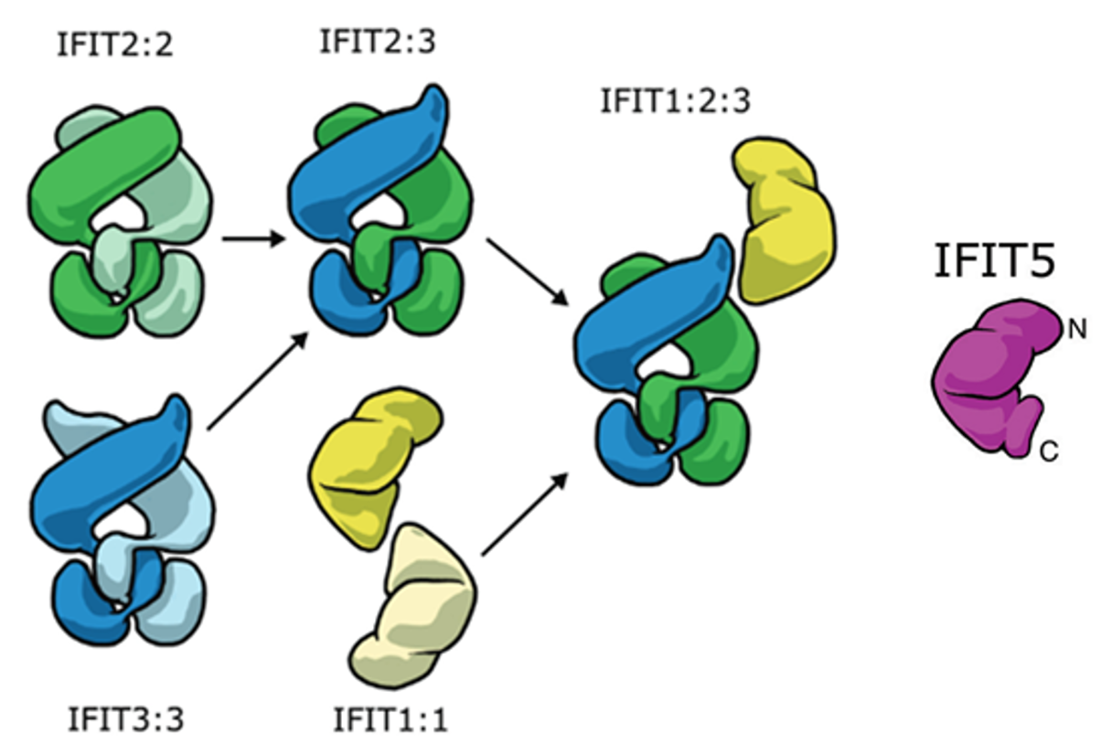
\includegraphics[width=0.75\linewidth]{04. Introduction//Figs/05. IFIT-complexes.png}
    \caption[IFIT Structures and Multimer Formation.]{\textbf{IFIT Structures and Multimer Formation.} IFIT tertiary and quaternary protein conformations are illustrated. IFIT1 is shown in yellow, IFIT2 in green, IFIT3 in blue, and IFIT5 is highlighted in purple. IFIT1 is able to homodimerise or heterooligomerise with IFIT2 and IFIT3 via its C terminal domain. IFIT5 has the corresponding interaction domain occluded by a helix and thus does not interact with the rest of IFIT proteins. IFIT2 and IFIT3 are capable of forming homodimers or heterodimers by ‘swapping’ TPRs in their N terminal regions. By combining the interactions IFIT1:2:3 heterotrimer is formed. The figure was adapted from Mears, 2018 \cite{Mears2018BetterResponse}.}
    \label{fig:IFIT Structures and Multimer Formation.}
\end{figure}

\subsection{Localisation and Functions of IFIT Proteins} \label{subsec:Localisation and Functions of IFIT Proteins}
\subsubsection{Localisation of IFIT Proteins} \label{Localisation of IFIT Proteins}
To date, IFIT protein localisation has been has been well studied in human and mouse models. Most publications indicate IFITs to be predominantly cytoplasmic. In more detail, nascent murine Ifit1 and human IFIT1 have been observed to localise diffusely in the cytoplasm while being excluded from the nucleus in NIH3T3 and P2.1 cell lines respectively \cite{Pichlmair2011IFIT1RNA, Terenzi2008Interferon-inducibleE1}. The human protein atlas, utilising two distinct anti-IFIT1 antibodies, indicates IFIT1 to have granular cytoplasmic and nuclear localisation in A431 and U2OS cells; and cytoplasmic, nuclear-excluded localisation in HeLa cells \cite{Thul2017AProteome}. IFIT2 reported localisation in the literature yields inconsistent results. While nascent murine Ifit2 was observed to be cytoplasmic while also associated with the mitotic spindle in all phases of the cell cycle in NIH3T3 and B16F10 cell lines \cite{Saha2006IdentificationProtein}, exogenously expressed human IFIT2 was reported to be cytosolic and thus excluded from mitochondria in HeLa cell line \cite{Stawowczyk2011TheApoptosis}. The latter is in conflict with what the human protein atlas reports on a nascent IFIT2 localisation in HeLa and U2OS cell lines, wherein both report cytoplasmic vesicular localisation distribution \cite{Thul2017AProteome}. IFIT3 has been indicated to localise cytoplasmically, with the evidence arising from exogenous overexpression experiments in THP-1 and HEK293T cells, with the latter further confirming IFIT3 colocalizing with mitochondria \cite{Huang2008Interferon-inducedCells, Liu2011IFN-InducedTBK1}. The human protein atlas confirms these findings by reporting nascent IFIT3 to show granular cytoplasmic localisation with partial nuclear staining in A431 and HeLa cell lines \cite{Thul2017AProteome}. Lastly, there is a discrepancy with regard to IFIT5 subcellular localisation. While exogenously expressed IFIT5 has been observed to localise at the ruffled membrane at the cell surface and to colocalise with actin-rich protrusions from the apical cell surface in both fibroblast-derived WI-38 VA-13 and hepatocyte-derived Huh7 cell lines \cite{Katibah2013TRNAIFIT5}, the human protein atlas reports nascent IFIT5 display granular cytoplasmic localisation with partial nuclear localisation and concentrations resembling the Golgi apparatus in A431 and SK-MEL-30 cell lines \cite{Thul2017AProteome}. 

\subsubsection{Inhibition of Translation and Viral Replication} \label{Inhibition of Translation and Viral Replication}
IFITs can restrict viral replication by several mechanisms. IFIT1 and IFIT5 can physically prevent non-self RNA from interacting with eukaryotic initiation factor (eIF) 4F \cite{Kumar2014InhibitionMRNAs}. IFIT1 and 2 block the binding of eIF3 to the eIF2-GTP-Met-tRNA ternary complex by interacting with the eIF3E subunit, whereas human IFIT2, and mouse IFIT1 and IFIT2, can block the formation of the 43S-mRNA complex by binding to the eIF3C subunit \cite{Diamond2014IFIT1:Translation, Guo2000CharacterizationVirus}. This is a cap-independent mechanism for viral translation inhibition, however, extensive IFIT expression can negatively influence the whole cellular translation processes via this mechanism and can hinder normal inflammatory responses. Overexpression of IFIT1 in human embryonic kidney (HEK) 293T cells inhibited the activation of IRF3 and NF\(\kappa\)B and the transcription of IFN\(\beta\) in response to polyinosinic-polycytidylic acid (poly I:C) \cite{Li2009ISG56Response}. The previously mentioned affinity of IFIT2 for AU-rich RNA can also regulate cellular translation as a lot of transcripts for cytokines or apoptotic factors are rich in adenine and uracil \cite{Palanisamy2012ControlMicroRNAs}. 

\subsubsection{Modulation of Innate Immune Response Signalling} \label{Modulation of Innate Immune Response Signalling}
IFIT proteins also have the potential to influence innate immune responses by direct interaction with signalling cascade proteins. IFIT3 can potentiate RIG-I signalling by forming a scaffold between MAVS and TANK-binding kinase 1 (TBK1), \cite{Liu2011IFN-InducedTBK1}, whereas IFIT5 enhances this pathway upstream by recruiting RIG-I to MAVS \cite{Zhang2013IFIT5Pathways}. IFIT5 has also been reported to help facilitate NF\(\kappa\)B activation via scaffolding its activation kinases \cite{Zhang2013IFIT5Pathways}. On the other hand, studies show that IFIT1 can both negatively and positively influence RIG-I signalling, upstream of MAVS. IFIT1 interacts with the stimulator of interferon genes (STING), an enhancer of MAVS and TBK1 interaction and it was proposed that these conflicting actions are caused by its multiple binding sites on STING \cite{Li2009ISG56Response, Reynaud2015IFIT1Interferon}. 

\subsubsection{Effects on Cell Cycle Progression and Apoptosis} \label{Effects on Cell Cycle Progression and Apoptosis}
IFIT2 and IFIT3 also have roles in cellular homeostasis. IFIT2 overexpression induces the mitochondrial dependent apoptotic pathway. IFIT2 has been shown to localise on mitochondrial membranes and to directly interact with pro-apoptotic factors which lead to apoptosome formation and subsequent caspase-9 activation \cite{Chen2017InhibitionApoptosis, Diamond2013TheProteins}. Expression of IFIT3 has been observed to alleviate these effects, most probably by the formation of IFIT2:3 dimers \cite{Mears2018BetterResponse, Stawowczyk2011TheApoptosis}. IFIT3 has also been observed to have negative effects on proliferation via indirect degradation of cyclin-dependant kinase inhibitor p27. As a result, cell cycle progression halts at the G1/S transition checkpoint \cite{Xiao2006RIG-GProteins}. An overview of the IFIT mechanisms of action is depicted in Figure \ref{fig:Overview of IFIT Mechanisms of Action}.

Therefore, IFITs not only act as complementary RNA sensors to RIG-I but are also important as mediators of a plethora of other processes. These range from regulation of transcription, activation and inhibition of innate immune signalling, and regulation of cell life cycle. It is again possible that preference for these actions is influenced by the levels of particular IFIT proteins and their interplay. Taking into consideration the above-described modes of IFIT expression activation, we can speculate that different stimuli such as viruses or signalling molecules at different concentrations will result in quite diverging actions of IFIT proteins on the phenotype of the cell.

\begin{figure}
    \centering
    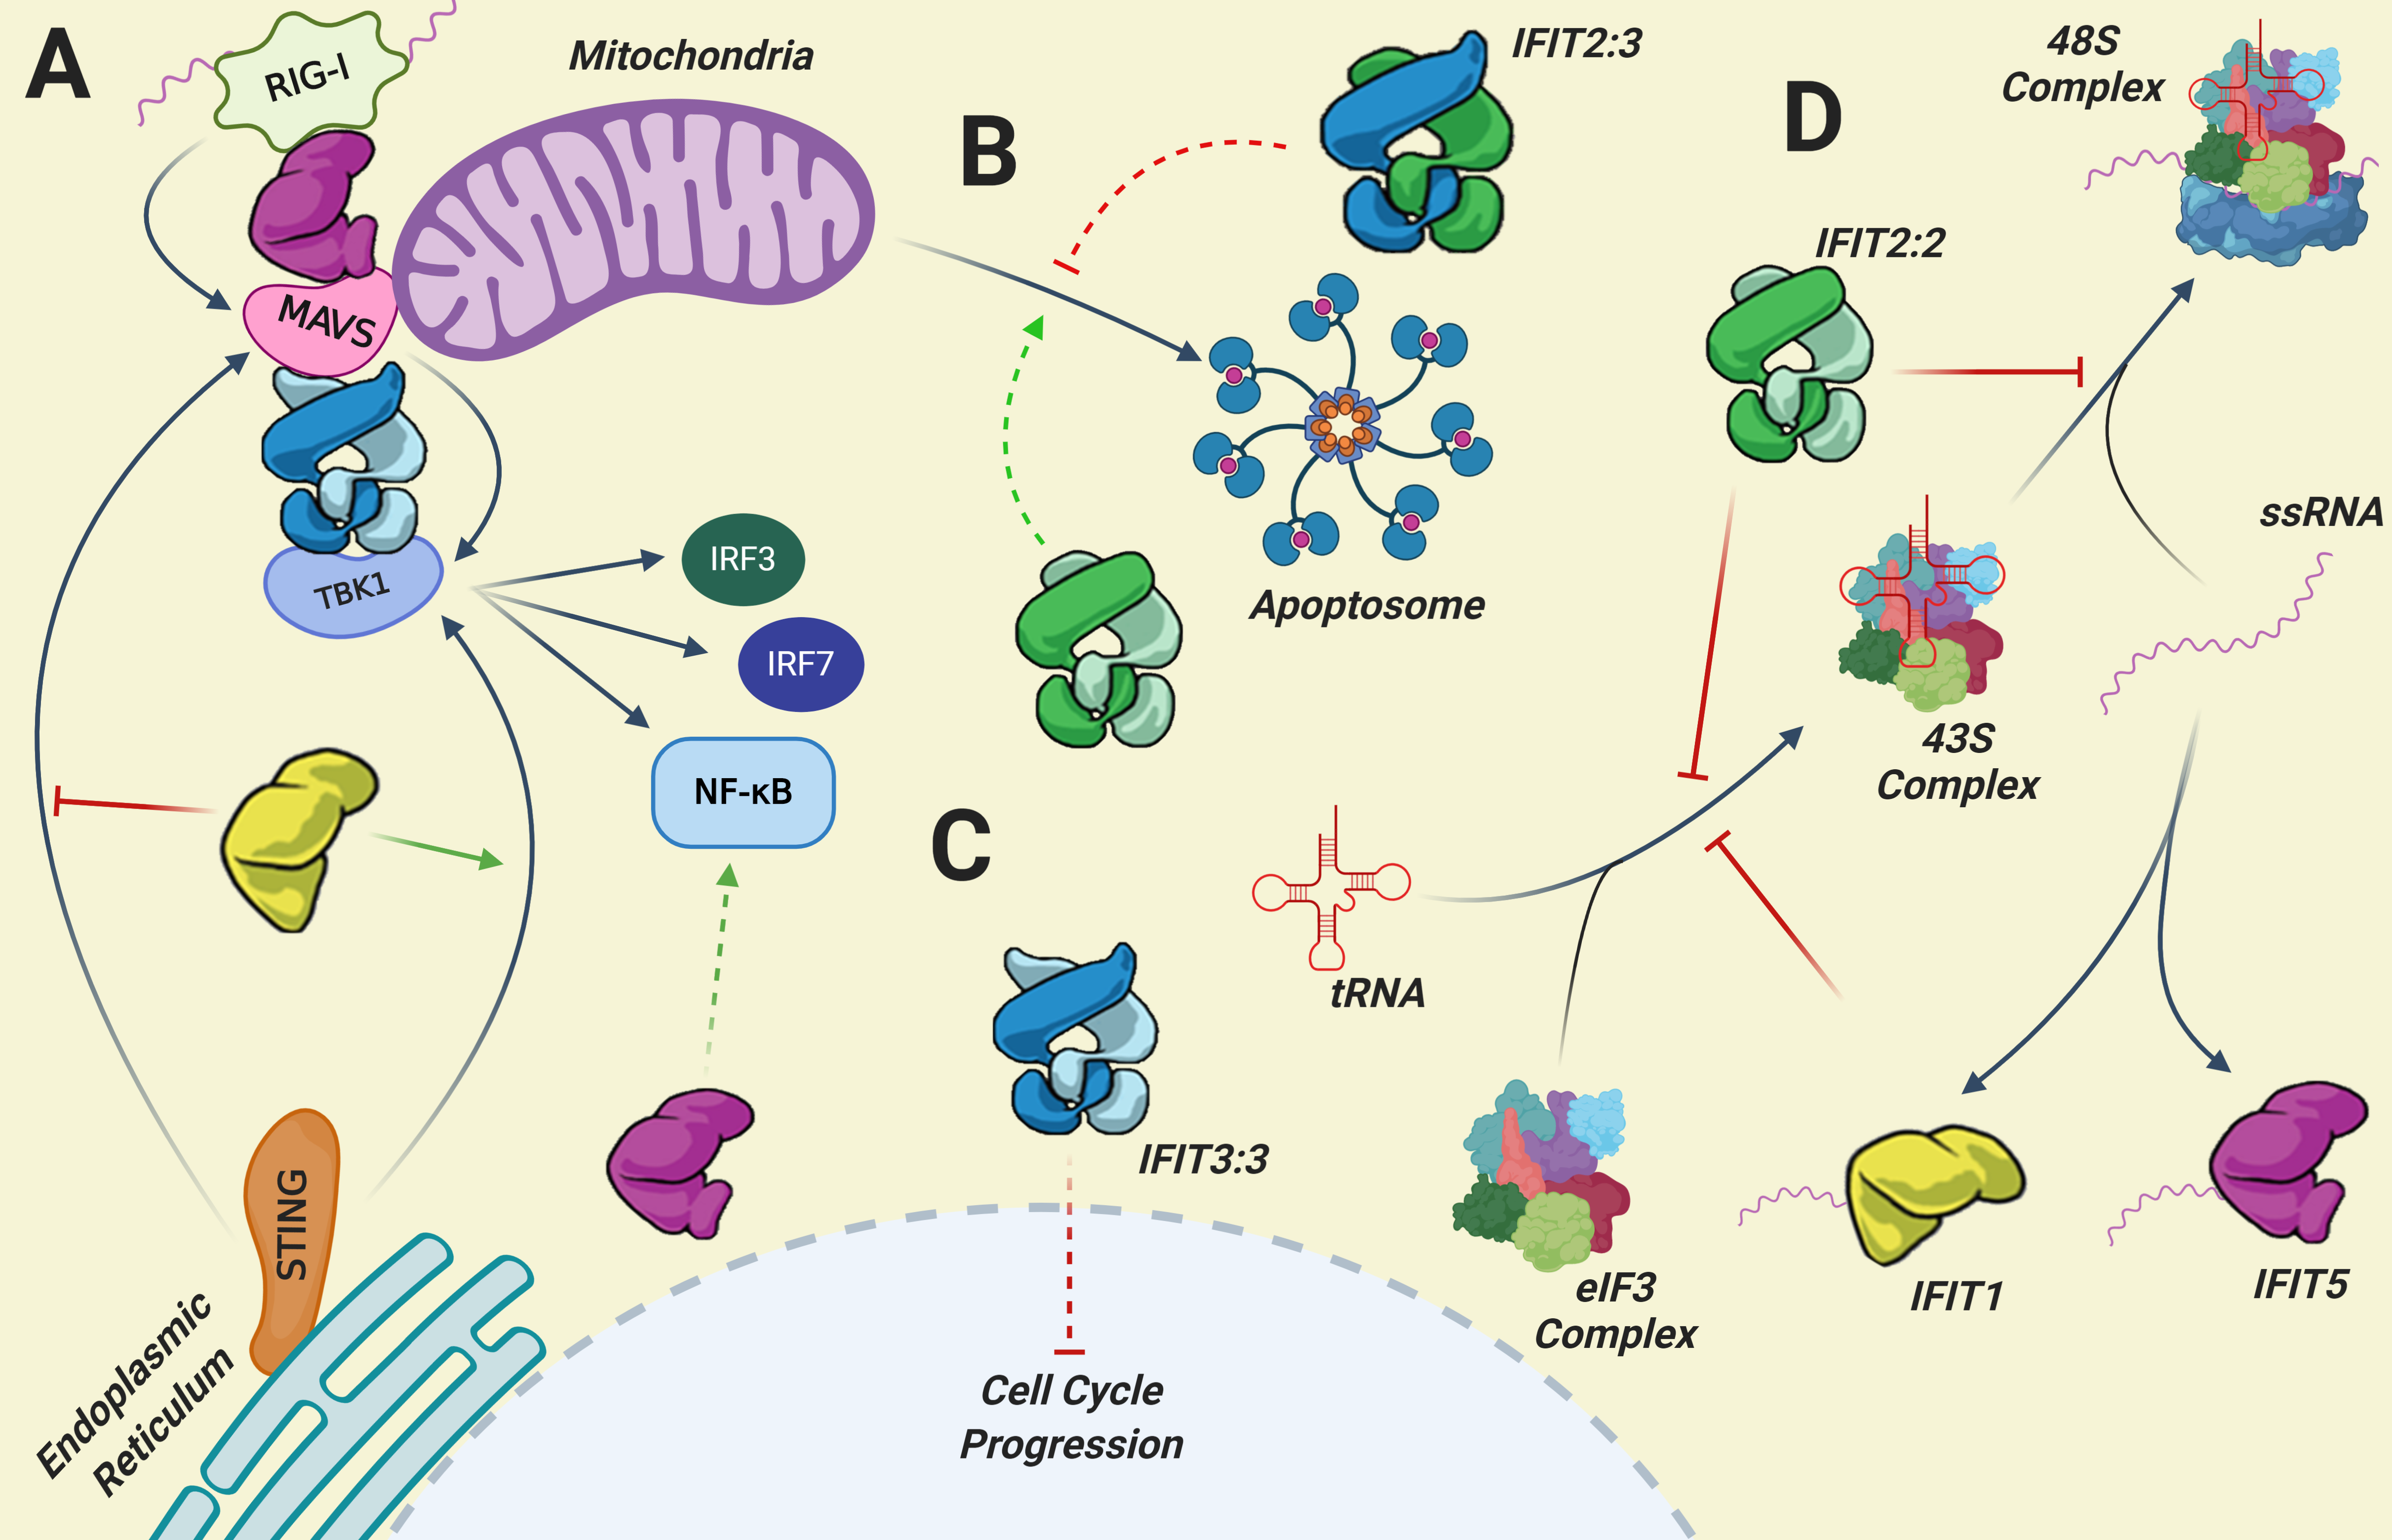
\includegraphics[width=1\linewidth]{04. Introduction//Figs/06. IFIT Mechanism of Action.png}
    \caption[Overview of IFIT Mechanisms of Action.]{\textbf{Overview of IFIT Mechanisms of Action.} IFITs have been described to have multiple actions in cells. Pathway A shows their involvement in innate immune signalling modulation. IFIT5 potentiate RIG-I activation of MAVS by scaffolding the two proteins together. IFIT3:3 further scaffolds MAVS to its effector, TBK1, which induces IRF3, IRF7 and NF\(\kappa\)B nuclear translocation when activated. STING protein also potentiates MAVS and TBK1 interaction. IFIT1 has been observed to inhibit STING interaction with MAVS while potentiating its interaction with TBK1. IFIT5 can also indirectly activate NF\(\kappa\)B. Pathway B shows IFIT2:2 involvement with apoptosome formation. IFIT2:3 complex reduces the pro-apoptotic activity of IFIT2:2. IFIT3:3 is involved in cell cycle arrest, as depicted in pathway C. Pathway D shows IFIT inhibition of viral replication and cellular translation. IFIT1 and IFIT5 can directly bind to cap0 and 5’PPP mRNA respectively and prevent its translation. IFIT1 and IFIT2 can both prevent 43S complex formation, while IFIT2 can also inhibit 48S complex formation. IFIT, Interferon-Induced Protein with Tetratricopeptide Repeats; RIG-I, retinoic acid-inducible gene I; MAVS, mitochondrial antiviral signalling protein; TBK1, TANK-binding kinase 1; STING, stimulator of interferon genes; IRF, interferon regulatory factor; NF\(\kappa\)B, nuclear factor kappa B; eIF, eukaryotic elongation factor; ssRNA, single-stranded RNA; tRNA, transfer RNA. The figure was adapted from Mears, 2018 \cite{Mears2018BetterResponse} and Diamond, 2013 \cite{Diamond2013TheProteins}. Created using BioRender.com.}
    \label{fig:Overview of IFIT Mechanisms of Action}
\end{figure}

\subsection{IFIT Responses to Viral Infections} \label{subsec:IFIT Responses to Viral Infections}
Human IFIT effects on single-stranded RNA viruses have been studied extensively within the past decade. \cite{Rabbani2016Identification3} reported that IFIT1 and IFIT3 restrict human parainfluenza virus 3 (PIV3, negative-sense ssRNA virus), while ectopic expression of IFIT2 and IFIT5 did not affect the viral fitness. \textit{In vitro} IFIT1 knock-down experiments using short hairpin RNA showed marked enhancement of protein expression of human PIV2, PIV5, and mumps virus, all negative-sense ssRNA viruses \cite{Andrejeva2013ISG56/IFIT1Synthesis, Young2016HumanFamily}. Hantaviruses, a family of negative-sense ssRNA viruses such as Prospect Hill virus (PHV), and Tula virus (TULV), strongly induce IFIT3 expression during the course of their infection \cite{Matthys2011TheInduction}. Most importantly within the non-segmented negative-sense ssRNA viruses, IFIT1, IFIT2, and IFIT3 have been reported to be globally antiviral against respiratory syncytial virus (RSV). Dori and colleagues either overexpressed or silenced these 3 IFITs and assessed RSV fitness by quantifying the viral mRNA produced. They reported decreased viral fitness following overexpression, while silencing of IFITs increased the viral mRNA production \cite{Drori2020InfluenzaProteins}. Another negative-sense ssRNA virus, which bears a segmented genome, influenza A virus, has been shown to upregulate IFIT1, IFIT2, and IFIT3 in primary macrophages during infection \cite{Lietzen2011QuantitativeMacrophages}. Recent studies also show the ability of IFIT1 and IFIT2 to negatively influence the viral fitness of influenza, as the knock-down of these IFITs resulted in increased viral RNA and protein production, while the opposite was true if IFIT1 and IFIT2 were overexpressed \cite{Zhu2023TheSynthesis}. Human IFIT1 has been observed to be differentially expressed during hepatitis C virus (HCV) infection. HCV was described to suppress IFIT1 upregulation and subsequent experiments showed an inverse relationship between artificial levels of IFIT1 and HCV ability to infect host cells \cite{Raychoudhuri2011ISG56Replication, Ishida2019HepaticInfection}. Currently, there is very limited information about the effect of bovine IFIT expression on the viral fitness of bovine viruses.


\section{Respiratory Syncytial Virus} \label{sec:Respiratory Syncytial Virus}
Human and bovine Respiratory Syncytial Viruses (hRSV and bRSV) are enveloped, negative-sense, single-stranded RNA viruses belonging to the Orthopneumovirus genus \cite{Afonso2016Taxonomy2016}. These viruses are recognized for inducing acute respiratory disease, which is confined to their respective hosts. Despite this host specificity, shared genetic and antigenic characteristics are observed among these closely related viruses \cite{Buchholz2000ChimericVaccine}. hRSV primarily infects humans, while bRSV infects cattle. They are known to be the leading causes of lower respiratory tract illness in their respective hosts \cite{Nair2013GlobalAnalysis, Sacco2014RespiratoryCattle}. Although these viruses can infect individuals of all ages, severe respiratory illness, including bronchiolitis and pneumonia, is more common in infants, the elderly, and immunocompromised individuals \cite{Falsey2005RespiratoryAdults, Coultas2019RespiratoryAge}. On a global scale, hRSV affects nearly all children by the age of five, resulting in approximately 35 million cases and 3.5 million hospital admissions annually in the United States of America \cite{Shi2017GlobalStudy}. Tragically, around 60,000 hospitalized children under the age of five succumb to the infection, with a notably higher mortality rate among infants under six months, especially those at high risk due to factors such as premature birth and pre-existing chronic lung and heart conditions \cite{Shi2017GlobalStudy, Jha2016RespiratoryVirus, Coultas2019RespiratoryAge}. Bovine RSV infection also poses a significant threat to the global cattle farming industry, resulting in substantial economic losses \cite{Brodersen2010BovineVirus, Valarcher2007BovineInfection}.

Despite extensive research and development efforts spanning several decades, the availability of approved vaccines against hRSV remains limited. Historical challenges include the failure of the formalin-inactivated RSV vaccine, which led to enhanced natural infection in some vaccinated children \cite{Fulginiti1969RespiratoryVaccine., Kim1969RespiratoryVaccine.}. Additional hurdles involve the heterogeneity of RSV subtypes and the incomplete immune responses generated against the virus. However, recent advances in the field have introduced a range of vaccine strategies, including live-attenuated wild-type virus, vector-based, viral protein sub-unit, mRNA-based, and DNA-based candidates. Presently, 24 vaccines are in various stages of clinical development, including two licensed vaccines: Arexvy (GSK) and Abrysvo (Pfizer). These vaccines are used as immunizing agents to prevent lower respiratory tract disease in older adults, with Abrysvo additionally indicated for passive immunization of infants through maternal administration during pregnancy \cite{Topalidou2023RespiratoryVaccines}. In contrast, there are several vaccines available for bRSV, with the first one dating back to the 1970s. However, these vaccines offer only mild protection. Consequently, there is a pressing need to develop more efficacious vaccines for both hRSV and bRSV \cite{Ellis2017HowCattle}.

\subsection{Genomic and Virion Composition} \label{subsec:Genomic and Virion Composition}
The size of the RNA genome of human and bovine RSV is reported to be 15,223 nucleotides for hRSV A2 subtype and 15,140 nucleotides for bRSV A51908 subtype, as reported by GenBank (GenBank identifiers KT992094 and NC038272 respectively). The RSV genome contains ten genes in the order 3'-NS1-NS2-N-P-M-SH-G-F-M2-L-5' (Figure \ref{fig:The Composition of RSV Virion and Genome}, panel b), which are transcribed into 10 monocistronic, capped, methylated, and polyadenylated mRNAs \cite{Collins2013RespiratoryDisease, Bohmwald2016HumanPathology}. These encode for 11 proteins as \textit{M2} gene is composed of two overlapping open reading frames (ORFs), which are accessed by coupled translation, where the ribosomes translating the first ORF (M2-1) move a short distance upstream after termination and reinitiate translation from a second (M2-2) overlapping ORF \cite{Gould2007CouplediPneumovirinae/i}.

RSV virions were observed to be pleomorphic, confronting to spherical (circa 100 nm radius), asymmetric, and filamentous (circa 5 \(\mu\)m in length) structures, as observed by electron microscopy, with a conserved structural organisation \cite{Kiss2014StructuralComplex}. Virions produced in cell culture are predominantly observed to be filamentous in several cell types leading to a hypothesis stating that the spherical and asymmetric particles are the breakdown and aggregation by-products of filamentous particles \cite{Ke2018TheTomography, Conley2022HelicalVirus}. Within an \textit{in vitro} context, a substantial portion (95\%) of the progeny virus persists attached to the cell surface, appearing as particles that have seemingly undergone incomplete budding. The standard procedure for cultivating virus stocks involves subjecting infected cells to processes such as sonication, freeze-thawing, or vortexing, aimed at detaching the virus. It is important to note, however, that these methods lead to a reduction in infectivity and an increase in the risk of cellular contamination \cite{Collins2013RespiratoryDisease}.

A representative filamentous RSV virion, based on the current literature, is depicted in Figure \ref{fig:The Composition of RSV Virion and Genome}, panel a. It is composed of the structural proteins, which include F, G, SH, M, M2-1, N, P and L proteins. M2-1 (transcription processivity factor) and matrix (M) proteins form subsequent lattice structures which support the viral membrane and dictate the filamentous shape of the virion \cite{Conley2022HelicalVirus}. The attachment (G) and fusion (F) glycoproteins are embedded in the viral membrane and helically ordered in pairs, as dictated by the M lattice. The small hydrophobic (SH) protein is also embedded in the membrane \cite{Ke2018TheTomography, Conley2022HelicalVirus}. Inside the virion resides nucleocapsid which is composed of RSV genomic RNA-bound within the groves nucleoprotein (N) multimeric protein complexes. These have been observed to be found in two forms, either as a polymer of helical nucleocapsid, which spans several RSV genomes in its structure (Figure \ref{fig:Nucleocapsid Polymer and Its Interaction with Viral RNA}) \cite{Tawar2009CrystalVirus, Conley2022HelicalVirus} or double-decameric N-RNA rings \cite{Gonnin2023StructuralNucleocapsids, Gonnin2022ImportanceVirus, Conley2022HelicalVirus}. These further interact with the large polymerase subunit (L) and the phosphoprotein polymerase cofactor (P) to form the ribonucleoprotein complex (RNP) \cite{Gonnin2023StructuralNucleocapsids}. The P stabilises the RNP structure with the virion by interacting with M2-1 protein \cite{Mason2003InteractionActivity}.

\begin{figure}
    \centering
    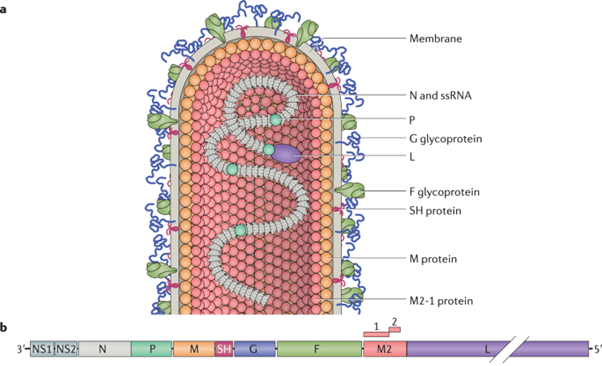
\includegraphics[width=1\linewidth]{04. Introduction//Figs/07. RSV-composition.png}
    \caption[The Composition of RSV Virion and Genome.]{\textbf{The Composition of RSV Virion and Genome.} a) The most biologically correct diagram of the filamentous RSV virion is depicted. M2-1 (transcription processivity factor) and matrix (M) proteins form subsequent lattice structures which support the viral membrane and dictate the filamentous shape of the virion. The attachment (G) and fusion (F) glycoproteins are embedded in the viral membrane and helically ordered in pairs, as dictated by the M lattice. The small hydrophobic (SH) protein is also embedded in the membrane. Inside the virion, a helical nucleocapsid is present, composed of viral RNA genome-bound nucleoprotein (N) polymer, with its precise protein structure shown in grey. The large polymerase subunit (L) and the phosphoprotein polymerase cofactor (P) are also associated with N. b) The human RSV genome from the A2 strain is shown to scale. it contains 10 genes encoding 11 proteins, with the M2 gene encoding the M2-1 and M2-2 proteins. ssRNA; single-stranded RNA. Figure taken from Battles, 2019 \cite{Battles2019RespiratoryIt} and the structural biology basis for this figure is from Conley, 2022 \cite{Conley2022HelicalVirus}.}
    \label{fig:The Composition of RSV Virion and Genome}
\end{figure}

\begin{figure}
    \centering
    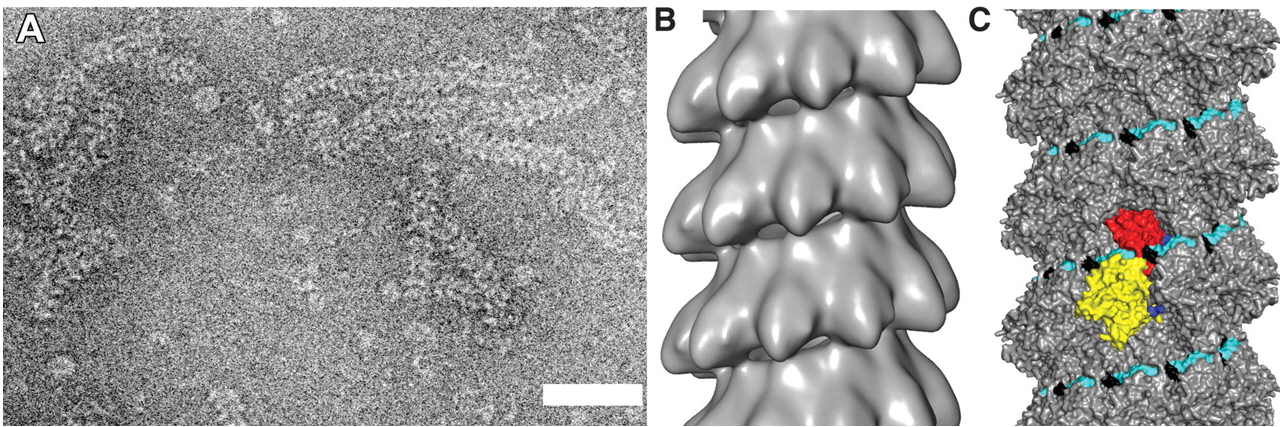
\includegraphics[width=1\linewidth]{04. Introduction//Figs/08. N-structure.jpeg}
    \caption[Nucleocapsid Polymer and Its Interaction with Viral RNA.]{\textbf{Nucleocapsid Polymer and Its Interaction with Viral RNA.} Panel A shows a negative-stained electron micrograph of recombinant RSV nucleocapsid-like helices. The scale bar indicates 50 nm. Panel B presents the 26 \r{A}-resolution 3D reconstruction of the observed helices formed by the nucleocapsid polymer. A single helix comprises 9.8 N subunits per turn. Panel C provides a more detailed view of the structure, with the encapsulated RNA shown in cyan and one N protein labelled based on its domains, with the N-terminal domain coloured in yellow and the C-terminal domain coloured in red. Figure adapted from Tawar, 2009 \cite{Tawar2009CrystalVirus}.}
    \label{fig:Nucleocapsid Polymer and Its Interaction with Viral RNA}
\end{figure}

\subsection{The Function of RSV Proteins} \label{subsec:The Function of RSV Proteins}
Both F and G are the main antigenic proteins of RSV \cite{Collins2011ProgressYears, Battles2019RespiratoryIt}. The F protein is involved in viral entry and assembly. It is generated as an inactive F0 precursor in the cytoplasm, after which it is activated by furin-like proteases in the Golgi apparatus \cite{Collins1984NucleotideVirus.}. The active form of the F protein in the viral particles is a trimer in a prefusion conformation \cite{Ternette2007ImmunogenicityVirus}. The fusion protein has been reported to interact with several host surface receptors, such as toll-like receptor 4 (TLR4) \cite{Marr2012RoleReplication}, intercellular adhesion molecule-1 (ICAM-1) \cite{Behera2001BlockingInfection}, or nucleolin, with the latter believed to be the main RSV receptor and determinant of viral tropism \cite{Tayyari2011IdentificationVirus}. The G protein is not vital for successful infection and is present in two forms, either as a membrane-bound form or a secreted isoform. Membrane-bound G enhances F protein binding to cellular surface receptors by facilitating membrane attachment via the interaction with heparin and annexin 2 \cite{Collins2013RespiratoryDisease, Krusat1997Heparin-dependentCells, Malhotra2003IsolationCells}, while the secreted form is responsible for immune system evasion by antibody binding saturation \cite{Bukreyev2008TheLeukocytes}. 

The transmembrane SH protein, situated as well at the virion surface, forms pentameric pore-like structures that exhibit cation-selective channel-like activity \cite{Carter2010DirectPermeability, Gan2012TheChannels}. While the significance of this activity for RSV remains unclear, the SH protein is identified as a viroporin, belonging to a category of small viral proteins capable of modifying membrane permeability and influencing processes such as budding and apoptosis. Reports suggest that SH has a modest effect in reducing apoptosis via the interaction with B-cell receptor-associated protein 31 (BAP31), as documented by \cite{Fuentes2007FunctionProtein}. Moreover, SH appears to inhibit signalling from TNF-\(\alpha\), an antiviral cytokine \cite{Fuentes2007FunctionProtein}. Recombinant RSV lacking SH demonstrates a somewhat more efficient \textit{in vitro} replication compared to the wild-type virus, possibly attributed to its smaller genome size and reduced number of genes. Additionally, this SH-deficient variant shows a slight attenuation in both mice and chimpanzees \cite{Whitehead1999RecombinantChimpanzees}. It has been observed for \(\Delta\)SH RSV virus infection to result in enhanced tumour necrosis factor (TNF) signalling and increased production of IL-1\(\beta\), which could explain the observations mentioned above \cite{Pollock2017ModulationProtein}. 

In this context, the primary function of the non-structural proteins NS1 and NS2 appears to be the modulation of innate immune responses, achieved through various documented mechanisms. The NS proteins of RSV play a crucial role in disrupting host innate immunity by forming a "Nonstructural degradosome complex", acting as a proteasome-like entity that degrades numerous proteins involved in the innate immune system \cite{Boyoglu-Barnum2019BiologyDevelopment.}. Studies involving single- and double-gene-deleted NS mutant RSV infections (\(\Delta\)NS1, \(\Delta\)NS2, or \(\Delta\)NS1/2) have demonstrated that both proteins function individually and collaboratively to achieve a comprehensive inhibitory effect on type I and III interferons, with NS1 exhibiting a more individual role \cite{Sedeyn2019RespiratoryResponses, Spann2004SuppressionMacrophages}. Cytosolic NS1 exhibits a propensity to translocate to the host nucleus and interact with the gene regulatory domains of immune response genes, thereby influencing gene transcription and modulating the host response against RSV infection \cite{Pei2021Nuclear-localizedTranscription}. NS1 localized to mitochondria inhibits type-I interferon (IFN) signalling by binding with mitochondrial antiviral signalling protein (MAVS), as the MAVS-RIG-1 complex is essential for type-I IFN activation \cite{Boyapalle2012RespiratoryInfection}. NS1 also stimulates miR-29a expression, affecting mRNA coding for interferon alpha/beta receptor 1 (IFNAR1) \cite{Sedeyn2019RespiratoryResponses, Zhang2016RespiratoryReceptor}. The NS1 protein interferes with the activation of the IFN gene promoter by inhibiting the phosphorylation of interferon regulatory factor 3 (IRF-3) has been documented \cite{Spann2005EffectsCytokines}. Similarly, NS2 can interfere with the activation of IRF-3 through its interaction with retinoic acid-inducible gene 1 (RIG-I), inhibiting the activation of IFN response genes (IFNRs) \cite{Wright2006TheHumans}. The NS1 protein is capable of interrupting the signalling of JAK/STAT pathways activated by IFN receptor pathways, particularly through the degradation of STAT2 \cite{Wright2006TheHumans, Sedeyn2019RespiratoryResponses}. Both NS1 and NS2 proteins can promote phosphoinositide 3-kinase (PI3K) pathways, enhancing the survival of infected cells and increasing viral yield \cite{Wu2012TheBiology.}. Additionally, NS2 plays a significant role in modulating cell morphology, leading to the shedding of infected cells and the increased dissemination of RSV virions \cite{Sedeyn2019RespiratoryResponses, Liesman2014RSV-encodedObstruction}. Recombinant RSV lacking the NS1 and/or NS2 genes displays heightened sensitivity to interferon, increased apoptosis, and reduced replication efficiency in both cultured cells and experimental animals, with the impact of deleting NS1 being more pronounced \cite{Whitehead1999RecombinantChimpanzees, Teng2000RecombinantChimpanzees}.

The M protein assumes a crucial role in the morphogenesis of virions through its interactions with the cell membrane, viral envelope, and viral nucleocapsid \cite{Li2008AssociationProtein, Marty2003AssociationCells}. Although not imperative for the initiation of viral filament formation, the absence of M results in stunted and immature filaments, highlighting its significant contribution \cite{Mitra2012TheFilaments}. During the early stages of infection, M is detected in the nucleus and may modestly inhibit host transcription during RSV infection. Subsequently, M is found associated with cytoplasmic viral inclusion bodies (IBs), presumed sites of viral RNA synthesis, and the plasma membrane, which serves as the location for virion formation \cite{Ghildyal2006CentralInfection}. M seems to play a role in suppressing viral RNA synthesis by nucleocapsids, likely in preparation for their packaging into virions, \cite{Ghildyal2006CentralInfection, NarayanTalukdar2022RespiratoryVirus}. Additionally, M is deemed necessary for the transport of nucleocapsids from viral inclusion bodies to the plasma membrane \cite{Mitra2012TheFilaments, Collins2013RespiratoryDisease}.

M2-2 functions as an accessory protein and, although not indispensable for virus growth, is expressed at a low level in infected cells \cite{Cheng2005OverexpressionReplication, Melero2006MolecularVirus}. However, its precise status as a virion component remains unknown \cite{Collins2013RespiratoryDisease}. Deletion of M2-2 from recombinant RSV results in a virus displaying delayed and reduced RNA replication along with increased "runaway" transcription. This is in contrast to wild-type RSV, where transcription appears to be downregulated later in infection in favor of RNA replication. These findings suggest that M2-2 plays a crucial role in regulating RNA synthesis. Specifically, as the level of M2-2 increases during the course of infection, it is associated with a reduction in transcription and a concurrent promotion of RNA synthesis \cite{Teng1998IdentificationParticles}.

\begin{figure}
    \centering
    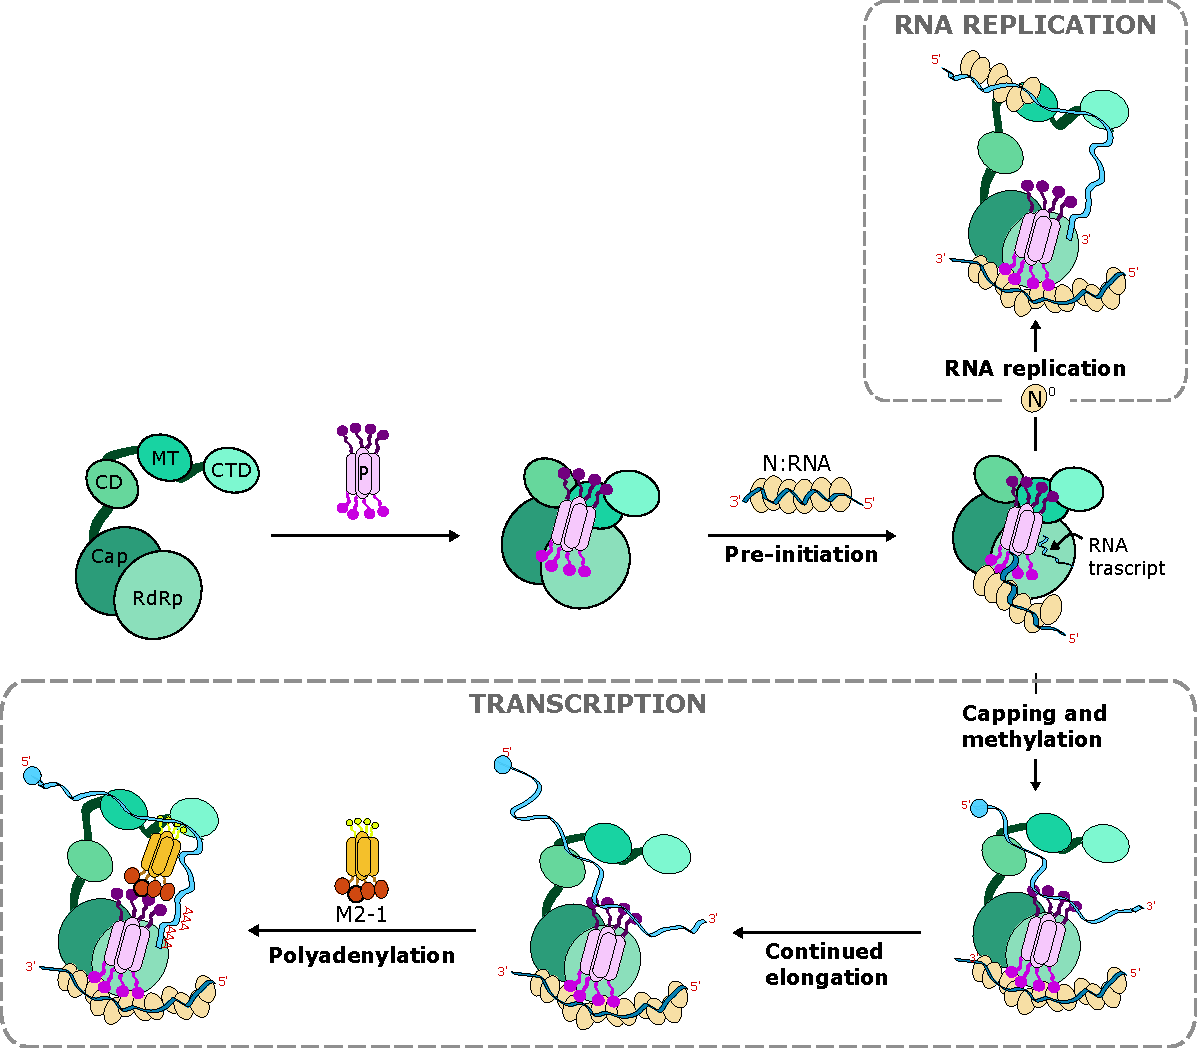
\includegraphics[width=1\linewidth]{04. Introduction//Figs/09. N_p_l_m21-interaction-overview.pdf}  
    \caption[A Model of RNP-Mediated RSV RNA Transcription and Replication.]{\textbf{A Model of RNP-Mediated RSV RNA Transcription and Replication.} The L protein, composed of the connector domain (CD), the methyltransferase domain (MT), the C-terminal domain (CTD), the Cap domain, and the RdRp domain, undergoes conformational rearrangement after interacting with tetrameric P protein in the pre-initiation step. During the initiation stage, the nucleocapsid, composed of N polymer bound to the RSV RNA template, is recruited by interaction with P protein. This causes a partial liberation of the RNA template and allows L to access it. If the RNA transcription follows, the Cap and the MT domains rearrange to catalyze the cap addition and cap methylation. Afterwards, the elongation stage of the transcription continues until the transcript polyadenylation step, which is mediated by M2-1 recruitment. Upon the supply of the N° (RNA-free N), the RNA replication continues. Figure adapted from Cao, 2021 \cite{Cao2021StructuralComplexes}.}
    \label{fig:A Model of RNP-Mediated RSV RNA Transcription and Replication}
\end{figure}

The M2-1 protein, an integral component of the RNP complex, acts as an antitermination/elongation factor, facilitating the transcription of all hRSV genes, thereby assisting the L protein in transcribing viral genes \cite{Collins1996TranscriptionVirus., Noton2015InitiationReplication}. Predominantly localized within cytoplasmic viral inclusion bodies (IBs) formed during infection \cite{Rincheval2017FunctionalVirus}, M2-1 exists in phosphorylated and nonphosphorylated forms. Both forms interact with the P protein, with phosphorylation dictating binding partners, localization (cytoplasmic or intra-IB), and subsequent function \cite{Richard2018RSVTranscription}. Phosphorylated M2-1 in the cytoplasm interacts with P bound to phosphatase PP1, facilitating dephosphorylation and recruitment into IBs, where they regulate viral mRNA transcription \cite{Richard2018RSVTranscription}. Subsequently, M2-1 binds and concentrates with newly synthesized mRNA, displacing P \cite{Blondot2012StructureProtein.}. Phosphorylation then releases M2-1 from mRNA designated for translation, allowing free M2-1 to potentially initiate the cycle anew by interacting with P \cite{Richard2018RSVTranscription}. As mentioned in Section \ref{subsec:Genomic and Virion Composition}, the N protein associates with RSV genomic RNA to form the nucleocapsid, exhibiting either as a long helical polymer or a decameric ring structure \cite{Gonnin2023StructuralNucleocapsids}. This configuration protects the genome from cellular RNA sensors and RNAses \cite{Tawar2009CrystalVirus}, compartmentalizing and concentrating it within RSV inclusion bodies where N localizes \cite{Rincheval2017FunctionalVirus}. These structures house other RNP components (M2-1, P, and L), facilitating efficient RSV RNA translation and replication. The RSV L protein, a single polypeptide of 2165 residues, serves as the catalytic core of the RSV polymerase, bearing distinct enzymatic domains (RdRp, Cap, and MT) and structural domains (CD and CTD) \cite{Gilman2019StructureComplex, Cao2020Cryo-EMPolymerase}. Its principal role involves the replication and transcription of the viral genome, regulated and supported by the RNP complex. The L protein directly transcribes the genome into mRNA for the expression of each hRSV gene \cite{Cowton2006UnravellingSynthesis, Noton2015InitiationReplication}. During replication, the L protein converts the entire virus genome from negative-sense RNA to positive-sense RNA (antigenome), which serves as a template for generating new negative-sense RNA encapsulated in virions \cite{Cowton2006UnravellingSynthesis, Fearns2000FunctionalVirus}. A characteristic feature of the L protein is its ability, during transcription, to create a gradient of gene expression from 3' to 5', resulting in a higher production of mRNAs for genes located 3' compared to those at 5' in the genome \cite{Hardy1998TheTranscription, Kuo1996TheMinigenome}. The phosphoprotein (P) acts as a cofactor for the RNP complex, serving as a multimodular adaptor for RNA synthesis through interactions with N-RNA, L, and M2-1 \cite{Blondot2012StructureProtein., Cardone2021APhosphoprotein}. It facilitates N protein interaction, allowing access to L \cite{Sourimant2015FinePhosphoprotein} and acts as a chaperone for newly synthesized, RNA-free N monomer (N0) protein. The N0-P complex prevents N0 association with host RNA, delivering them to nascent RSV genomes or antigenomes \cite{Castagne2004BiochemicalDomain, Galloux2015IdentificationNucleoprotein}. A proposed model of sequential RSV RNA synthesis suggests that P coordinates L activity, revealing a previously unappreciated role for L domain arrangements. Upon binding, a tetrameric P locks CD, MT, and CTD domains of L into a closed conformation (pre-initiation). This complex recruits N:RNA to form an initiation complex, initiating \textit{de novo} RNA synthesis. The domains adopt an open conformation upon promoter recognition, remaining open during elongation, resulting in increased mobility of CD, MT, and CTD domains of L. Depending on N°, RNA synthesis proceeds to transcription (capping and methylation, continued elongation, and polyadenylation) or replication \cite{Cao2020Cryo-EMPolymerase} (Figure \ref{fig:A Model of RNP-Mediated RSV RNA Transcription and Replication}).
































\subsection{RSV Inclusion Bodies} \label{subsec:RSV Inclusion Bodies}


 
% functions
Analysis of hRSV infected cells by immunofluorescence (IF) microscopy shows concentration of several viral proteins within IBs including N, P, L, M2-1, M and NS2 (Carromeu et al., 2007, Garcia et al., 1993, Lindquist et al., 2010, Brown et al., 2005, McDonald et al., 2004, Ghildyal et al., 2002). Most of these viral proteins are directly/indirectly associated with the nucleocapsid, explaining their colocalization within the structure. Interestingly, all of the proteins involved in transcription and replication (N, P, L and M2-1) co-localise in the IBs, whereas the surface glycoproteins are excluded. Recent identification of viral genomic RNA and mRNA within the IB (Fig 1.9) strongly suggests that these organelles are functional and are the primary site for viral RNA replication and transcription within the infected cell (Rincheval et al., 2017). Interestingly, distinct spatial organisations were observed between viral genomic and mRNA. As already noted above, mRNA concentrated in IBAGs whereas genomic RNA mostly localised towards the boundary of the IB (Fig 1.9). Further study is required to understand the significance of this organisation. Similarly, IBs produced in rabies (Lahaye et al., 2009) and ebola (Hoenen et al., 2012) virus infected cells were also shown as the sites of RNA replication and transcription. However, this does not appear to be universal a trend since viral RNA replication of Nipah virus (NiV) was recently shown to occur outside both its structurally distinct IB populations (Ringel et al., 2019). As discussed in sub-section 1.2.3, a number of host cell proteins have been shown to interact with or co-localise within RSV induced IBs. These include antiviral proteins MAVS and MDA5 (Lifland et al., 2012), and signalling proteins involved in the cellular response to viral infection – p38 mitogen-activated protein kinase (MAPK) and O-linked N-acetylglucosamine transferase (OGT) (Fricke et al., 2013). In addition, the chaperone protein, HSP70 that protects cells from stress, has also been observed within RSV IBs (Brown et al., 2005). MDA5 and MAVS sequestration into IBs were shown to result in a reduction of IFNβ mRNA induction (Lifland et al., 2012). Similarly, sequestration of p38 MAPK and OGT suppressed MK2 activity and stress granule assembly. Recruitment of these key signalling proteins into IBs following RSV infection appears to be an additional mechanism of immune antagonism whereby their roles are inhibited through sequestration. + the 2 FJ papers

and the subunit p65 of NF-KB









% fj 2020 paper
The cytoplasmic inclusion bodies induced by hRSV infection share many characteristics with liquid organelles or biomolecular condensates (24-26) having similarity to stress granules, P-bodies, and nucleoli. They are also structurally and functionally similar to viral inclusions formed by rabies, human metapneumovirus, and measles viruses (27-30) and likely represent an essential component of the life cycle of many negative-sense RNA viruses. For the pneumoviruses, these membraneless organelles have been shown to contain N, P, L, and M2-1 (26, 29-31), which are viral proteins involved in viral genome replication and mRNA transcription, together with the M protein. Importantly, the presence of viral genomic RNA and mRNA within the IB strongly suggests that these organelles are functional and are the primary site for viral RNA replication within the infected cell (26). 


% fj 2023 paper
IBs formed during infection have dynamic properties and host a multitude of viral-viral and viral-host protein interactions underpinning a diverse range of functions [20-23]. The best characterised is the concentration of viral proteins for the spatio-temporal compartmentalisation of viral RNA replication and mRNA transcription [16-18, 24].

We and others have also previously shown that IBs are highly organised, with newly synthesised mRNA and the RNA-binding M2-1 protein [18, 27] further compartmentalised into sub-IB droplets, termed inclusion body-associated granules (IBAGs) [17, 18, 27]. The presence of poly(A)-binding protein (PABP) and the translation initiation factor eIF4G in these mRNA-rich droplets [17] suggests a role in translation initiation [28]. Although it has been suggested that IBAG contents are released into the cytoplasm for viral translation to occur [17], there is little information available on the ultimate site for translation of RSV viral mRNAs.

% talk about assembly and llps and ibags
% about ib sizes
\cite{}
% n and p interaction

 Co-expression of the N and P proteins alone results in the formation of IB-like structures (pseudo-IBs) with similar properties to the viral inclusions. The minimal system however does not rule out the involvement of RNA interactions in formation of the structures as cellular RNA may be used in the absence of virus infection. More recently, the N and P proteins of RSV (Galloux et al., 2020b) and MeV (Guseva et al., 2020) were shown to induce liquid droplets outside of the cellular environment, thus showing they are the main drivers of viral phase separation. However, there was a discrepancy between the two viruses in cells as the formation of pseudo-IBs by RSV N and P required N:RNA interaction (Galloux et al., 2020b); however, the MeV proteins did not (Guseva et al., 2020, Zhou et al., 2019). Guseva et al. further showed that although RNA is dispensable for MeV N:P phase separation, it preferentially colocalises to and triggers assembly of nucleocapsid-like particles within the structures formed. Similar to cellular proteins involved in inducing LLPS, assembly of ectopically expressed N and P proteins into inclusions has been shown to involve oligomerisationand intrinsically disordered domains within these viral proteins (Zhou et al., 2019, Nikolic et al., 2017, Galloux et al., 2020a). The higher degree of intrinsic disorder within P proteins of RSV (Gilman et al., 2019, Pereira et al., 2017), MeV and rabies virus (Nevers et al., 2020, Longhi et al., 2017) suggests it has a greater propensity to phase separate but the involvement of N shows there are crucial mechanisms provided by this protein. Mechanistically, for RSV, the central oligomerisation domain and C-terminal domain (an intrinsically disordered region) of P, plus the ability of N to interact with both P and RNA, were shown to be required for pseudo-IB formation (Galloux et al., 2020b). Of note, several other viral protein-protein and protein-RNA interactions which could contribute towards maturation exist in IBs. For instance, the viral nucleocapsid which concentrates in IBs (Fig 1.8 and Fig 1.9), is composed of genomic RNA, N, L and P proteins (Fig 1.2) (Easton et al., 2004). M2-1 also can form multiple interactions - with P (Mason et al., 2003, Richard et al., 2018), M (Li et al., 2008) and viral mRNA (Rincheval et al., 2017).

For RSV and related viruses, ectopic coexpression of the N and P proteins alone results in the formation of IB-like structures, indicating a evolutionarily conserved mechanism for IB formation (\cite{Lifland2012HumanMAVS}, \cite{Rincheval2017FunctionalVirus}, \cite{Nikolic2017NegriOrganelles}, \cite{Garca1993CytoplasmicProtein}).

However, the process of maturation appears to be a complex and regulated process as indicated by the organisation of the condensates into multi-phasic structures. Rincheval et al. recently demonstrated the presence of sub-compartments within RSV IBs with distinct protein and RNA composition, biophysical properties and functions termed inclusion body associated granules; IBAGs (Rincheval et al., 2017). M2-1 and newly synthesised viral mRNA, presumably interacting, mainly localised to these IBAGs (Rincheval et al., 2017). This is similar to the distinct, coexisting liquid phases that make up the nucleolus (Feric et al., 2016). The IBAGs are dynamic structures, and their contents are subsequently released to the cytoplasm.

% llps papers
\cite{Darling2023KnownCondensates} - membraneles condensates in general
\cite{Garabedian2022ProteinSequences} - protein condensates
\cite{Mohanty2022PrinciplesProteins} - principles of multidomain protein phase separation
\cite{Hu2022SequestrationPathological} - if cellular protein sequestration is pathological
\cite{Li2022PhaseInfections} - phase separation in viral infections
\cite{Dumelie2023BiomolecularMicroenvironments} - phospholipids concentrating in cellular and viral (sars2) inclusion bodies that seems to be passive


\cite{Rincheval2017FunctionalVirus} - ibags
\cite{Risso-Ballester2023SpatialBodies} - chapter about rsv ibs
\cite{Whelan2016FunctionalDisorder} - Functional correlations of respiratory syncytial virus proteins to intrinsic disorder
\cite{Weber1995NonstructuralSerum} - n p and ns2 inside ib (granular inclusion)
\cite{McDonald2004EvidenceAnalysis} - IBs accumulate touching the golgi apparatus -> lipid rafts of golgi

\begin{figure}
    \centering
    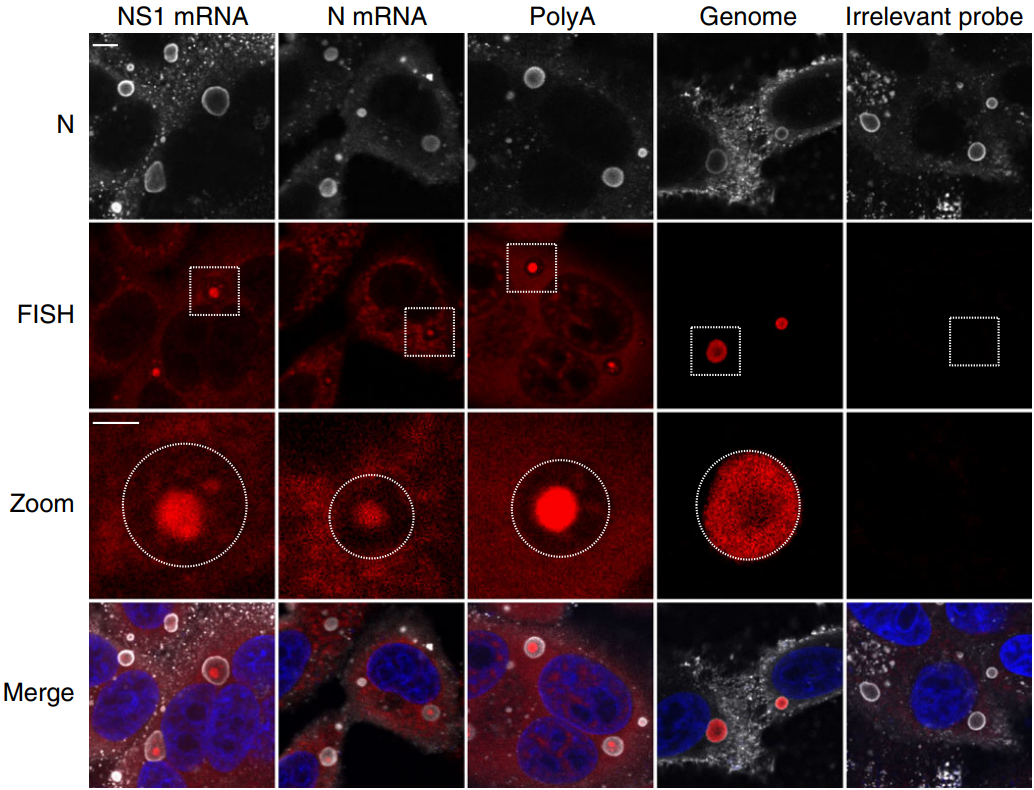
\includegraphics[width=1\linewidth]{04. Introduction/Figs/11. RSV IBs.png}  
    \caption[Viral RNA Discrete Localisation in hRSV Infected Cells.]{\textbf{Viral RNA Discrete Localisation in hRSV Infected Cells.} hRSV-infected HeLa cells were fixed 24 hours post-infection (HPI) and stained for the N protein (inclusion body identification) and specific RNA species using fluorescence \textit{in situ} hybridization (FISH). The latter were NS1 mRNA, N mRNA, polyadenylated RNA (PolyA), and viral genomic RNA which all localised within the inclusion body structures. Circles in the zoom panel represent IB boundaries. The scale bar in the top panel indicates 5 \(\mu\)m, while the one present in the zoom panel is 2 \(\mu\)m. Figure taken from Rincheval, 2017 \cite{Rincheval2017FunctionalVirus}.}
    \label{fig:Viral RNA Discrete Localisation in hRSV Infected Cells}
\end{figure}

% compartmalising rna replication
% immune suppresion - n mda and mavs; p56; new FJ paper


% ib sequesteration
\cite{Fricke2013P38Assembly} - p38 and got
\cite{Lifland2012HumanMAVS} - mavs and mda5
\cite{Jobe2020RespiratorySignaling} - NF-kB subunit p65
\cite{Jobe2023ViralCondensates} - the new paper

\cite{Brown2005EvidenceInfection} - ns2 protein inside IBS; HSP70 inside ibs; lipids in IBs (triacylglycerol and cholesterol-esters and taft lipids (GM1)); globular actin (G-actin) on the edge of ibs; 



% functions
Analysis of hRSV infected cells by immunofluorescence (IF) microscopy shows concentration of several viral proteins within IBs including N, P, L, M2-1, M and NS2 (Carromeu et al., 2007, Garcia et al., 1993, Lindquist et al., 2010, Brown et al., 2005, McDonald et al., 2004, Ghildyal et al., 2002). Most of these viral proteins are directly/indirectly associated with the nucleocapsid, explaining their colocalization within the structure. Interestingly, all of the proteins involved in transcription and replication (N, P, L and M2-1) co-localise in the IBs, whereas the surface glycoproteins are excluded. Recent identification of viral genomic RNA and mRNA within the IB (Fig 1.9) strongly suggests that these organelles are functional and are the primary site for viral RNA replication and transcription within the infected cell (Rincheval et al., 2017). Interestingly, distinct spatial organisations were observed between viral genomic and mRNA. As already noted above, mRNA concentrated in IBAGs whereas genomic RNA mostly localised towards the boundary of the IB (Fig 1.9). Further study is required to understand the significance of this organisation. Similarly, IBs produced in rabies (Lahaye et al., 2009) and ebola (Hoenen et al., 2012) virus infected cells were also shown as the sites of RNA replication and transcription. However, this does not appear to be universal a trend since viral RNA replication of Nipah virus (NiV) was recently shown to occur outside both its structurally distinct IB populations (Ringel et al., 2019). As discussed in sub-section 1.2.3, a number of host cell proteins have been shown to interact with or co-localise within RSV induced IBs. These include antiviral proteins MAVS and MDA5 (Lifland et al., 2012), and signalling proteins involved in the cellular response to viral infection – p38 mitogen-activated protein kinase (MAPK) and O-linked N-acetylglucosamine transferase (OGT) (Fricke et al., 2013). In addition, the chaperone protein, HSP70 that protects cells from stress, has also been observed within RSV IBs (Brown et al., 2005). MDA5 and MAVS sequestration into IBs were shown to result in a reduction of IFNβ mRNA induction (Lifland et al., 2012). Similarly, sequestration of p38 MAPK and OGT suppressed MK2 activity and stress granule assembly. Recruitment of these key signalling proteins into IBs following RSV infection appears to be an additional mechanism of immune antagonism whereby their roles are inhibited through sequestration. + the 2 FJ papers

and the subunit p65 of NF-KB


Furthermore, a number of host cell proteins involved in the antiviral response (NF-KB subunit p65 [18], MAVS and MDA5 [25], phosphorylated p38 and O-linked N- acetylglucosamine transferase [26]) are sequestered into IBs to prevent their function. Protein phosphatase 1 (PP1) recruitment to the IB has also been shown to be involved in important post-translational regulation steps in the viral life cycle [22].

















\section{Aims of the Study} \label{sec:Aims}
Here have a page of the aims.

A detailed comparative study of human and bovine IFITs and their interaction with RSV. Looking at their induction, expression, and changes in localisation. Looking at interaction with RSV IBs. Assessing the involvement of IFIT2 in the RSV life cycle.

For your Aims make sure these are very detailed, so 2 pages roughly. Not 3-4 bullet points of 2 lines each, which I have seen!

clearly human ifits are global restictors of hrsv. but is it relevant, do they get induced? can we isolate what is inducing them if so? 

are human ifits induced by brsv and thus have a potential to crossprotect from it?

does this reproduce in bifit with brsv and crossprotection from hrsv?

through what mechanism are ifits inhibitory? where are they located during infection?

do they interact with parts of rsv stuff?

is there a difference between ifits in interaction with these structures?






It is currently unknown if IFIT proteins interact with these structures. Given the well-described roles of IFITs in sensing viral RNA, it is possible that different IFITs may localise into IBs and IBAG, potentially interacting with viral RNA before the capping process takes place or directly interfere with the translational machinery. It is also possible that IFITs are restricted from accessing IBs by an unknown mechanism. Understanding these processes may reveal novel routes of increasing viral sensitivity to the innate immune response.







%acronyms
\nomenclature[z-DEM]{DEM}{Untranslated}

\nomenclature[z-IBAG]{IBAG}{IB-Associated Granule}
\nomenclature[z-IB]{IB}{Inclusion Body}
\nomenclature[z-BVDV]{BVDV}{Bovine Viral Diarrhoea Virus}
\nomenclature[z-HCV]{HCV}{Hepatitis C Virus}
\nomenclature[z-TULV]{TULV}{Tula Virus}
\nomenclature[z-PHV]{PHV}{Prospect Hill Virus}
\nomenclature[z-PIV3]{PIV3}{Parainfluenza Virus 3}
\nomenclature[z-STING]{STING}{Stimulator of Interferon Genes}
\nomenclature[z-TBK1]{TBK1}{TANK-Binding Kinase 1}
\nomenclature[z-HEK]{HEK}{Human Embryonic Kidney}
\nomenclature[z-eIF]{eIF}{Eukaryotic Initiation Factor}
\nomenclature[z-ssRNA]{ssRNA}{Single-Stranded RNA}
\nomenclature[z-TPR]{TPR}{Tetratricopeptide Repeat}
\nomenclature[z-IFIT]{IFIT}{Interferon-Induced Protein with Tetratricopeptide Repeats}
\nomenclature[z-ISG]{ISG}{Interferon-Stimulated Gene}
\nomenclature[z-UTR]{UTR}{Untranslated Region}
\nomenclature[z-IRSE]{IRSE}{Interferon-Stimulated Response Elements}
\nomenclature[z-STAT]{STAT}{Signal Transducer and Activator of Transcription}
\nomenclature[z-JAK]{JAK}{Janus Kinase}
\nomenclature[z-IRF]{IRF}{Interferon Regulatory Factor}
\nomenclature[z-ISGF3]{ISGF3}{Interferon-Stimulated Gene Factor 3}
\nomenclature[z-5'-PPP]{5'-PPP}{5'-Triphosphoate}
\nomenclature[z-m7G]{m7G}{7-Methyl Guanosine}
\nomenclature[z-dsRNA]{dsRNA}{Double-Stranded RNA}
\nomenclature[z-MAVS]{MAVS}{Mitochondrial Antiviral Signalling Protein}
\nomenclature[z-RIG-I]{RIG-I}{Retinoic Acid-Inducible Gene I}
\nomenclature[z-MDA5]{MDA5}{Melanoma Differentiation-Associated Gene 5}
\nomenclature[z-NF\(\kappa\)B]{NF\(\kappa\)B}{Nuclear Factor kappa B}
\nomenclature[z-RSV]{RSV}{Respiratory Syncytial Virus}
\nomenclature[z-PRR]{PRR}{Pattern Recognition Receptor}
\nomenclature[z-PAMP]{PAMP}{Pathogen-Associated Molecular Pattern}
\nomenclature[z-LPS]{LPS}{Lipopolysaccharide}
\nomenclature[z-TLR]{TLR}{Toll-Like Receptor}


%Words in text: 2625
%Words in headers: 112